\documentclass{ctexart}[UTF8]
\usepackage{dirtree}
\usepackage{listings}
\usepackage{xcolor}
\usepackage{graphicx}
\usepackage{enumerate}
\usepackage[a4paper]{geometry} 
\usepackage{amsmath,amsthm,mathtools,amssymb}
\usepackage{mathtools}
\usepackage{diagbox}
\usepackage{multirow,makecell}
\usepackage{float}
\usepackage{url}
\usepackage[nottoc]{tocbibind}
\usepackage{float}
\newcommand{\refe}[1]{Eq.\ref{#1}}
\newcommand{\reft}[1]{Theory.\ref{#1}\ }
\newcommand{\reff}[1]{图\ref{#1}\ }
\lstset{
 columns=fixed,
 numbers=left,                                        % 在左侧显示行号
 numberstyle=\tiny\color{gray},                       % 设定行号格式
 basicstyle=\small\ttfamily,
 frame=none,                                          % 不显示背景边框
 backgroundcolor=\color[RGB]{245,245,244},            % 设定背景颜色
 keywordstyle=\color[RGB]{40,40,255},                 % 设定关键字颜色
 numberstyle=\footnotesize\color{darkgray},           
 commentstyle=\color{gray}\ttfamily,                  % 设置代码注释的格式
 stringstyle=\rmfamily\slshape\color[RGB]{128,0,0},   % 设置字符串格式
 showstringspaces=false,
 breaklines=true,
 language=c++
}
\newtheorem{theorem}{Theory}[section]
\geometry{bottom=2cm,left=1cm,right=1cm}
\title{上机11}
\author{张配天-2018202180}
\begin{document}
    \maketitle
    \tableofcontents
    \clearpage
    \section{斐波那契堆}
    \subsection{问题描述}
    实现斐波那契堆的\textbf{插入、合并、提取最小}的操作。
    \subsubsection{输入}
    向斐波那契堆插入的节点(\textbf{键值为整数})。
    \subsubsection{输出}
    从斐波那契堆提取的最小节点。
    \subsection{算法思路}
    按照书上的伪代码: \begin{enumerate}
        \item 实现节点及其双链表的结构;
        \item 定义将节点添加入根链表$\_append$、将两个根链表合并$\_concat$、将一个根链表并为另一个的孩子$\_link$、从根链表删除一个根节点$\_delete$四项基本操作, 每个操作虽然涉及到斐波那契堆的根链表, 但其实其基本单元仍为节点;
        \item 实现斐波那契堆的$insert$、$union$、$consolidate$三个方法;
    \end{enumerate}
    \subsection{复杂度分析}
    使用摊还分析中的势能法分析其复杂度;首先定义整个斐波那契堆的势能函数为:\begin{equation}
        \Phi(H) = t(H) + 2m(H)
    \end{equation}
    \par 其中$t(H)$为$H$中根链表中的节点数, $m(H)$为$H$中已标记节点的和。在$|H|=0$时, $\Phi(H) = 0$, 同时在$|H|>0$时恒有$\Phi(H) > 0$, 因此摊还代价$\sum\hat{c_i} = \sum(c_i + \Phi(H_i) - \Phi(H_{i-1}))$永远是实际代价的的上界;
    接下来分析每一个操作的摊还代价:\begin{enumerate}[I.]
        \item \textbf{插入操作:}\begin{align*}
            t(H') &= t(H) + 1\\
            m(H') &= m(H)\\
            \Delta\Phi(H) &= (t(H')+2m(H')) - (t(H)+2m(H)) = 1\\
        \end{align*}
        又因为链表本身的插入操作代价为$O(1)$, 于是摊还代价为$O(1) + 1 = O(1)$;
        \item \textbf{合并操作:}\begin{align*}
            t(H) &= t(H1)+t(H2)\\
            m(H) &= m(H1)+m(H2)\\
            \Delta\Phi &= \Phi(H) - (\Phi(H1)+\Phi(H2)) = (t(H)+2m(H))-(t(H1)+2m(H1)+t(H2)+2m(H2)) = 0\\
        \end{align*}
        由于链表本身的合并操作代价为$O(1)$, 于是摊还代价为$O(1)+0 = O(1)$
        \item \textbf{提取最小操作:}\begin{align*}
            \Phi(H) &= t(H)+2m(H)\\
            \Phi(H') &\le D(n)+1+2m(H)\\
            \Delta\Phi &\le D(n)-t(H)
        \end{align*}
        因为$D(n) =  O(lgn)$, 又因为链表本身的抽取操作代价为$O(D(n)+t(H))$, 所以抽取最小节点的摊还代价为$O(D(n)+t(H)) - t(H) = O(D(n)) = O(lgn)$。
    \end{enumerate}
    \subsection{源代码}
    \lstinputlisting[language=python]{d:/repositories/Algorithm/Data Structure/Fibnacci_Heap.py}
    \subsection{运行截图}
    \begin{figure}[H]
        \centering
        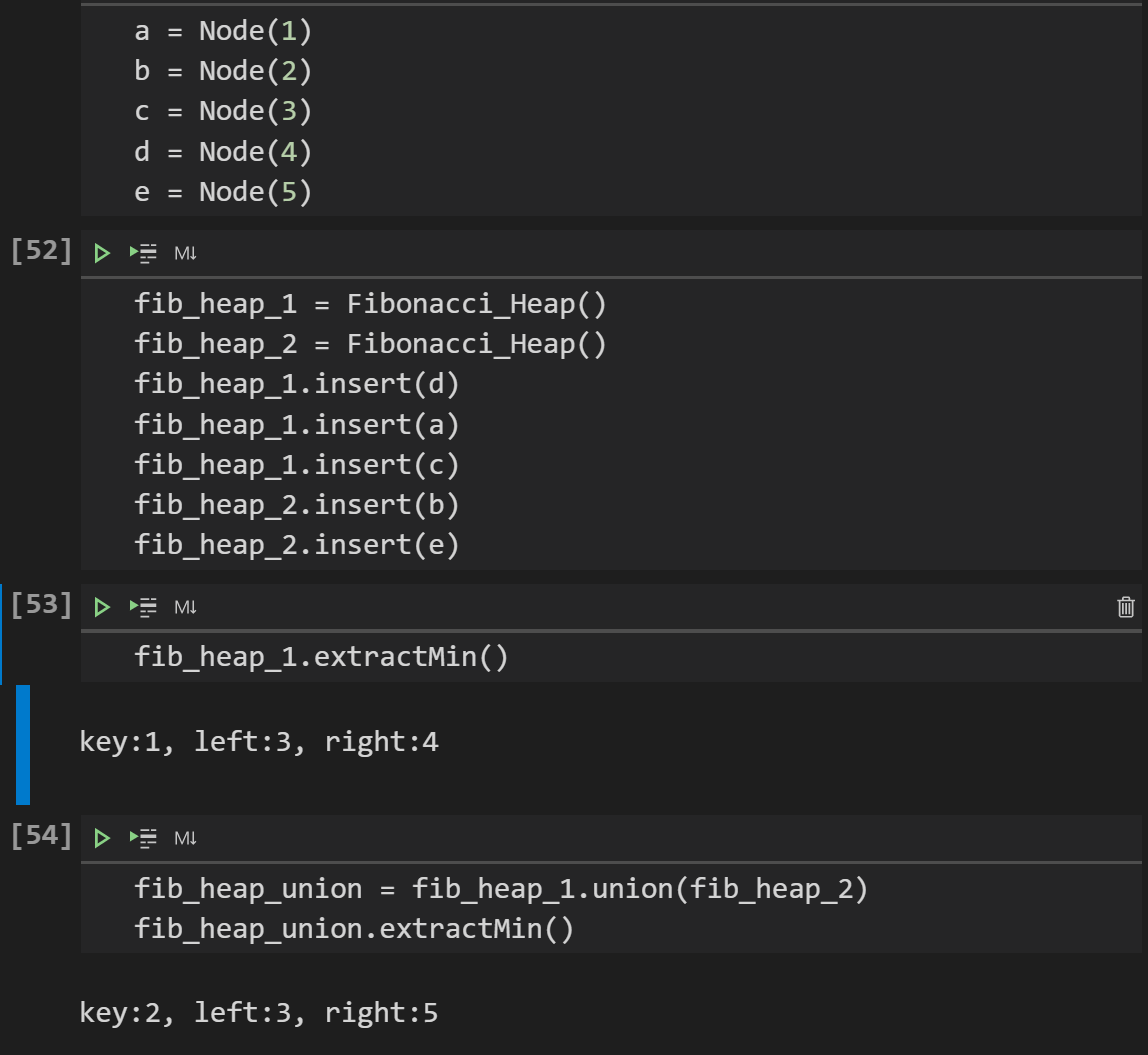
\includegraphics[width=12cm]{../Resources/11_1.png}
    \end{figure}
    可以看到, 运行正确。
\end{document}